\documentclass[12pt]{article}
\usepackage[utf8]{inputenc}
\usepackage[english]{babel} % Language to be used
\usepackage[T1]{fontenc}
\usepackage{amsmath}
\usepackage{amssymb}
\usepackage{amsthm}
\usepackage{cite}  % Package to cite multiple references at once
\usepackage{url}
\usepackage{hyperref}
\usepackage[usenames,dvipsnames]{xcolor}
\usepackage{listings}
\usepackage{float}
\usepackage{graphicx}
\usepackage{enumitem} 
%\usepackage{mathpazo}  Palatino-fonts
%\usepackage{txfonts}
\usepackage[stable]{footmisc}

\urlstyle{same} 


\lstset{
  basicstyle=\ttfamily,
  language=python,
  tabsize=4,
  frame=single,
  showstringspaces=false,
  showspaces=false,
  showtabs=false,
  captionpos=b,
  breaklines=true,
  breakatwhitespace=false,        % sets if automatic breaks should only happen at whitespace
  keywordstyle=\color{RoyalBlue},      % keyword style
  commentstyle=\color{ForestGreen},   % comment style
  stringstyle=\color{BrickRed}
}

\hypersetup{%
  colorlinks=true,    % hyperlinks will be black
  linkcolor=green,% hyperlink text will be green
  linkbordercolor=red,% hyperlink borders will be red
  pdfborderstyle={/S/U/W 1}% border style will be underline of width 1pt
}

% Parameters to the margins
\setlength{\topmargin}{-0.50in}
\setlength{\oddsidemargin}{-0.25in}
\setlength{\evensidemargin}{-0.25in}
\setlength{\textwidth}{7.0in}
\setlength{\textheight}{9.00in}

% Here is where all the new theorem environments are defined.
% Their use is described in the text.
\newtheorem{prop}{Proposition}
\newtheorem{thm}{Theorem}[section]
\newtheorem{lem}[thm]{Lemma}
\newtheorem*{Zorn}{Zorn's Lemma}

% Use a new style for definitions
\theoremstyle{definition}
\newtheorem{dfn}{Definition}

% Use a new style for remarks
\theoremstyle{remark}
\newtheorem*{rmk}{Remark}

\title{\centering{Notes to Hands-on Intro to R}}

\author{Wim R.\,M.\, Cardoen\\
	Center for High-Performance Computing (CHPC)\\
	University of Utah}


\begin{document}
\date{\today}
\maketitle
\thispagestyle{empty}
% ----------------------------------------------------------------
\pagestyle{plain}
\pagenumbering{arabic}
\setcounter{page}{1}
\renewcommand \thesection{\Roman{section}}

\section*{Section 6: $Z=X+Y$}
Let $X$ and $Y$ be random variables which are independent and have a uniform distribution in $[0,1]$.
Our goal is to find the cdf and pdf\footnote{cdf stands for the cumulative density function. pdf stands for the probability density function. 
If $f_X(x)$ is the pdf associated with the random variable $X$, then $F_X(X\le x):= \int_{-\infty}^x f_X(t) dt$ is the corresponding cdf.} for the random variable $Z=X+Y$. \newline
Their joint pdf $f_{X,Y}(x,y)$ (due to the independence of $X$ and $Y$) is given by:
\begin{eqnarray}
	f_{X,Y}(x,y) & = &f_X(x)\,f_Y(y) \nonumber \\
		     & = & \begin{cases}
			 1, & 0\le x \le 1\; \text{and} \;0\le y \le 1 \nonumber  \\
			     0, & \text{else}
		     \end{cases}    
\end{eqnarray}	
Thus, the random variable $Z$ can take on values in the interval $[0,2]$.
In order to derive the cdf and pdf for $Z$, we need to consider $2$ cases:
\begin{enumerate}
    \item $0\le z \le 1$
    \item $1 \le z \le 2$	    
\end{enumerate}		

\subsection*{Case $1$}
The cdf $F_Z(Z\le z)$, where $0\le z \le 1$ requires 
the calculation of the following integral:
\begin{eqnarray}
        F_Z(Z \le z) &= & \int_{x=0}^{x=z} \int_{y=0}^{y=z-x} f_{X,Y}(x,y)\,dx\,dy \nonumber \\
              & =& \frac{z^2}{2} \nonumber
\end{eqnarray} 
Due to the fact that the joint density function $f_{X,Y}(x,y)$ is $1$ within the area $0\le x \le 1\; , \;0\le y \le 1$ the 
aforementioned integral is identical to the area of the triangle with the following vertices:
$(0,0)$ and $(0,z)$ and $(z,0)$ (see Fig.\,\ref{case1})

\begin{figure}[H]
   \centering
	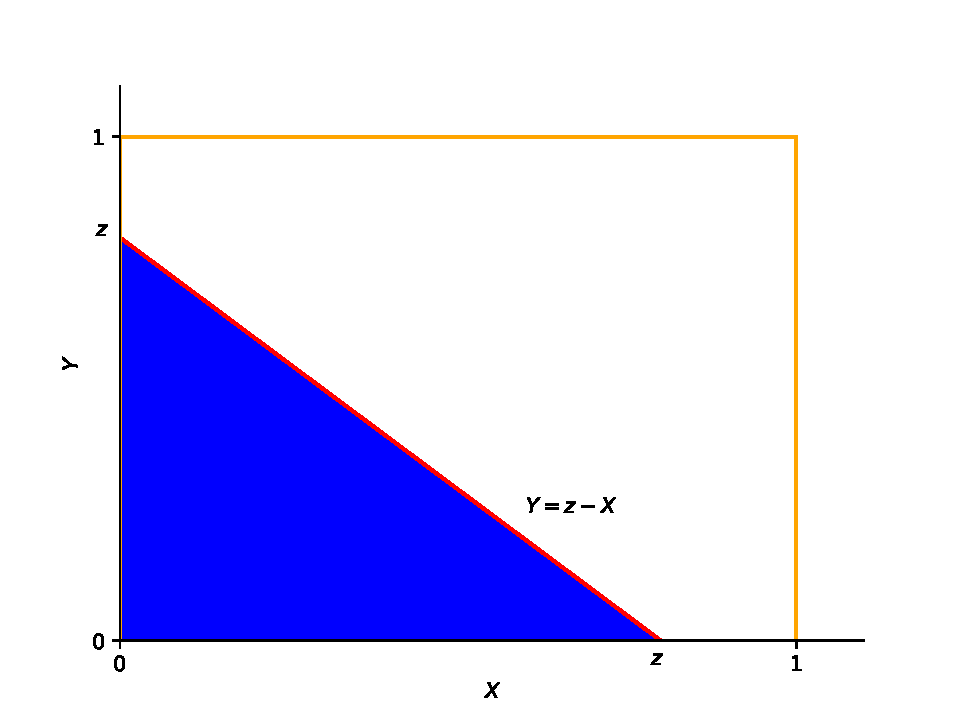
\includegraphics[width=0.95\textwidth]{../img/case1.pdf}
	\caption{$F_Z(Z \le z)$ is the area in blue ($0 \le z \le 1$)}\label{case1}
\end{figure}

\subsection*{Case $2$}
The cdf $F_Z(Z\le z)$, where $1\le z \le 2$ requires 
the calculation of the following integral (area in blue Fig.\,\ref{case2}). From Fig.\,\ref{case2}, it is quite obvious 
that the integral can be calculated a lot easier through its complement in probabilty (area in green):
\begin{eqnarray}
	\displaystyle F_Z(Z \le z) &= & 1 - \int_{x=z-1}^{x=1} \int_{y=z-x}^{y=1} f_{X,Y}(x,y)\,dx\,dy \nonumber \\
	      & =& 1-\frac{(2-z)^2}{2} \nonumber
\end{eqnarray} 



\begin{figure}[H]
   \centering
        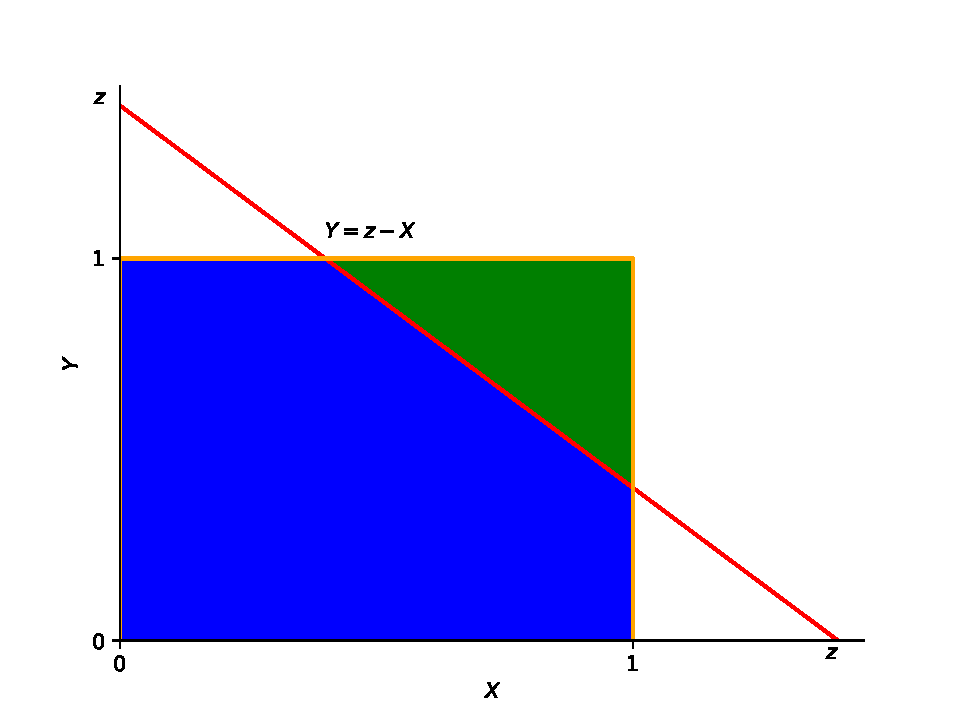
\includegraphics[width=0.95\textwidth]{../img/case2.pdf}
        \caption{$F_Z(Z \le z)$ is the area in blue ($1 \le z \le 2$)}\label{case2}
\end{figure}


\subsection*{Calculation of the pdf}
Above, we obtained the cdf $F_Z(z)$: 
\begin{eqnarray}
     F_Z(z) &= & \begin{cases}
                     \frac{z^2}{2} & 0 \le z \le 1 \nonumber \\
		     1 - \frac{(2-z)^2}{2} & 1 \le z \le 2 \nonumber \\
		     0   & \text{else} \nonumber
	         \end{cases}
\end{eqnarray}
From the cdf $F_Z(z)$ its pdf $f_Z(z)$ can be easily derived: 
\begin{eqnarray}
    f_Z(z) = \frac{d F_Z(z)}{dz} \nonumber
\end{eqnarray}	
The pdf $f_Z(z)$ thus becomes:
\begin{eqnarray}
     f_Z(z) &= & \begin{cases}
                     z   & 0 \le z \le 1 \nonumber \\
                     2-z & 1 \le z \le 2 \nonumber \\
                     0   & \text{else} \nonumber
                 \end{cases}
\end{eqnarray}



\end{document}
